\documentclass[tikz,border=4pt]{standalone}
\usetikzlibrary{positioning, shapes.geometric, arrows.meta}

\tikzset{
  base/.style     = {draw, thick, minimum width=28mm, minimum height=9mm, align=center},
  terminal/.style = {base, rounded corners=4.5mm, fill=teal!15},
  process/.style  = {base, fill=blue!8},
  decision/.style = {base, diamond, aspect=2.2, inner sep=1pt, fill=orange!15},
  io/.style       = {base, trapezium, trapezium left angle=70,
                     trapezium right angle=110, fill=gray!12},
  >={Stealth[length=2.5mm]},
}

\begin{document}
% Euclid's algorithm: the greatest common divisor of a and b.
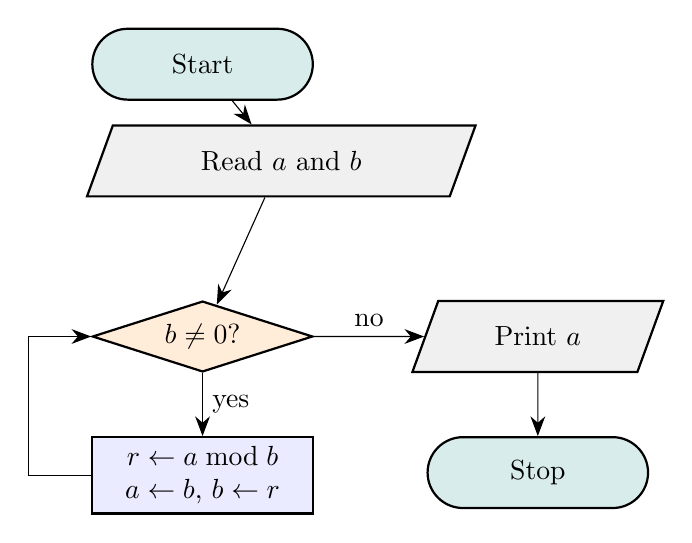
\begin{tikzpicture}[node distance=8mm and 14mm]
  \node[terminal]                (start) {Start};
  \node[io, below=3mm of start, xshift=1cm]      (read)  {Read $a$ and $b$};
  \node[decision, below=2.53cm of start] (test)  {$b \ne 0$?};
  \node[process, below=of test]  (step)  {$r \gets a \bmod b$\\ $a \gets b$, $b \gets r$};
  \node[io, right=of test]       (print) {Print $a$};
  \node[terminal, below=of print] (stop) {Stop};

  \draw[->] (start) -- (read);
  \draw[->] (read)  -- (test);
  \draw[->] (test)  -- node[right] {yes} (step);
  \draw[->] (test)  -- node[above] {no}  (print);
  \draw[->] (print) -- (stop);
  % The way back: out to the left, up, and into the test again.
  \draw[->] (step.west) -- ++(-8mm,0) |- (test.west);
\end{tikzpicture}
\end{document}
